\documentclass[border=6pt]{standalone}
\usepackage{pgfplots}
\pgfplotsset{compat=1.18}
\begin{document}
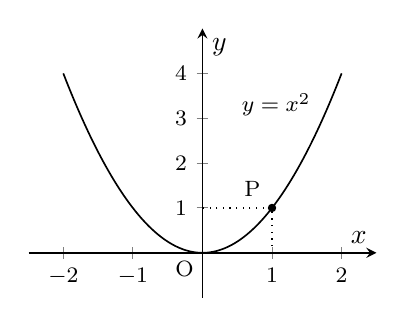
\begin{tikzpicture}[
  axisLabel/.style={font=\footnotesize,inner sep=1pt},
  pointLabel/.style={font=\footnotesize,inner sep=1pt},
  graphLabel/.style={font=\footnotesize,inner sep=1pt}
]
\begin{axis}[
  width=60mm,height=50mm,
  axis lines=middle,axis line style={-stealth,line width=0.60pt},
  xmin=-2.5,xmax=2.5,ymin=-1,ymax=5,
  xtick={-2,-1,1,2},ytick={1,2,3,4},
  xlabel={$x$},ylabel={$y$},clip=false,
  tick style={line width=0.35pt},tick label style={font=\footnotesize}
]
  \node[axisLabel,below left,xshift=-2pt,yshift=-2pt] at (axis cs:0,0) {$\mathrm{O}$};
  % gratik-domain-restricted: explicit example display interval [-2,2]
  \addplot[black,mark=none,samples=201,domain=-2:2,line width=0.60pt] {x^2};
  \draw[dotted,line width=0.40pt] (axis cs:1,0)--(axis cs:1,1)--(axis cs:0,1);
  \addplot[only marks,mark=*,mark size=1.3pt] coordinates {(1,1)};
  \node[pointLabel,above left,xshift=-3pt,yshift=3pt] at (axis cs:1,1) {$\mathrm{P}$};
  \node[graphLabel,anchor=west,xshift=3pt] at (axis cs:0.4,3.3) {$y=x^2$};
\end{axis}
\end{tikzpicture}
\end{document}
